\documentclass[a4paper,10pt]{article}

\usepackage{ucs}
\usepackage[utf8x]{inputenc}
\usepackage{amsmath}
\usepackage{amssymb}
\usepackage{subfigure}
\usepackage{fontenc}
\usepackage{graphicx}
\usepackage{capt-of}
\usepackage{natbib}
\bibliographystyle{apj.bst}
\usepackage{aas_macros}

\usepackage[dvips]{hyperref}

\date{03/15/15}

\begin{document}
 \section{Introduction}
 --Initial Problem (graph of obs data)\\
 --First thoughts (Hypothesis)\\
 \subsection{magnitude cut}
 Explanation for magnitude cut \label{magnitudecut}
 \section{Method}
 
 I simulate a synthetic stellar population using three variables to describe every given star: distance from earth ($r$), stellar mass ($M$) 
 and age ($t$). In accordance to the observational data I attempt to model, distance ranges from 0 to $r_{\mathrm{max}}=3\,$kpc and mass
 from $M_{\mathrm{min}}=5\,\mathrm{M}_\odot$ to $M_{\mathrm{max}}=50\,\mathrm{M}_\odot$. Because in first order the main sequence age 
 ($t_{\mathrm{ms}}$) of 
 a star is a strictly monotonic increasing function of $M$ one can define the maximum age for the oldest possible star in my sample to be
 $t_{\mathrm{max}}=t_{\mathrm{ms}}(M_{\mathrm{min}})$. With $M_{\mathrm{min}}=5\,\mathrm{M}_\odot$ and using equation 5 of 
 \citep*{2000MNRAS.315..543H} this translates to $t_{\mathrm{max}}\approx 104\,\mathrm{Myr}$.\\
 
 To formulate a probability density in fractional main sequence age ($\frac{dp}{d\tau}$), I need to know the probability densities for stars in space 
 $\left(\frac{dp}{dV}\right)$, mass 
 $\left(\frac{dp}{dm}\right)$ and age $\left(\frac{dp}{dt}\right)$. In my simulation I assume the stars are uniformly distributed in space. 
 Because of the radial symmetry of the problem, the distribution is solely dependant on the distance from earth,
 
 \begin{equation}
  \frac{dp}{dV}=\frac{1}{V_{\mathrm{tot}}}=\frac{1}{\frac43\cdot\pi\cdot r_{\mathrm{max}}^3}.
  \label{dpdV}
 \end{equation}
 
  I assume the stars are distributed in mass according to the Salpeter Initial Mass Function (IMF):
 $\frac{dp}{dM}=A\cdot M^{-2.35}$ \citep*{1955ApJ...121..161S}. Because the IMF follows an inverse power law, I use a logarithmic mass axis.
 Because of that I need to convert the IMF to a logarithmic binning using $d\log M = \frac{dM}{M\ln 10}$
 
 \begin{equation}
  \frac{dp}{d\log M}=\ln 10 \cdot A\cdot M^{-1.35},
 \end{equation}
 
 Where A is a normalization factor, that follows from: 
 
 \begin{equation}
  1=\int_{M_{\mathrm{min}}}^{M_{\mathrm{max}}}A\cdot M^{-2.35} dM =\left[ -1.35\cdot A\cdot M^{-1.35}\right]_{M_{\mathrm{min}}}^{M_{\mathrm{max}}},
 \end{equation}
 
 \begin{equation}
  A= \frac{1.35}{M_{\mathrm{min}}^{-1.35}-M_{\mathrm{max}}^{-1.35}}.
 \end{equation}
 
 I assume a constant star formation rate, so the probability density in age is $\frac{dp}{dt}=\frac{1}{t_{\mathrm{ms}}}$. 
 The age axis is also defined logarithmic to make sure massive stars with small $t_{\mathrm{ms}}$ are correctly represented.
 Because of this I need to find $\frac{dp}{d\log t}$ using $d\log t=\frac{dt}{t \ln 10}$; 

 \begin{equation}
  \frac{dp}{d\log t}=\frac{t\ln 10}{t_{\mathrm{ms}}}.
 \end{equation}

 With this information I can formulate the overall probability density function (PDF) for the stars in my sample with regard to $\tau$
 
 \begin{equation}
  \frac{dp}{d\tau}=\frac{dp}{dV}dV \cdot \frac{dp}{d\log t}d\log t \cdot \frac{dp}{d\log M}d\log M\cdot \frac{1}{d\tau}.
 \end{equation}
  
 
 To implement a magnitude cut I need to find the visual magnitude (V) for any given star. 
 The first step is to use analytical formulations derived from a stellar evolution model by \citet{2000MNRAS.315..543H} which approximates the
 stellar evolution as a function of initial mass ($M_{\mathrm{ini}}$), fractional main sequence age ($\tau$) and metalicity (Z).
 To do this, I need to find $\tau$. Equation 5 of \citep{2000MNRAS.315..543H} gives me the main sequence age for any given mass
 $t_{\mathrm{ms}}(M)$ and $\tau$ then becomes: $\tau(M)=\frac{t}{t_{\mathrm{ms}}(M)}$. I use Z=0.02 for all stars to simulate a metalicity
 similar to that of our sun according to \citet*{1998SSRv...85..161G}.
 I then use Equation 12 and 13 from the same paper to compute luminosity (L) and radius (R) for stars on the main sequence\footnote{
 \citet{2000MNRAS.315..543H} cites \citet*{1996MNRAS.281..257T} for Zero Age Mainsequence (ZAMS) Radii and Luminosities. 
 In Equation 1 of the cited paper there is a typo, where: $\gamma + M^3$ has to be $\gamma \cdot M^3$.}. \\
 
 Figure \ref{lumiradius} shows a Hertzsprung Russel Diagram (HRD) for five different stars on their main sequence based on the evolutionary
 model of \citet{2000MNRAS.315..543H}. To obtain temperature (T) I use the following equation with $\sigma$ being the Stefan-Boltzmann-Constant:
 
 \begin{equation}
  T=\sqrt[4]{L/(\sigma 4 \pi R^2)}.
 \end{equation}
 
  \begin{figure}[h!]
  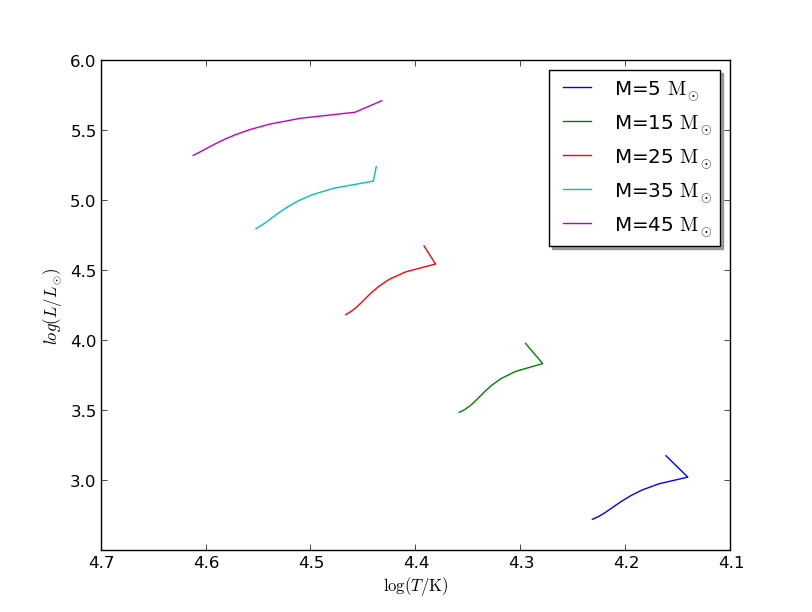
\includegraphics[width=\textwidth]{lumiradius}
  \caption{HRD for five different stars on their main sequence based on the evolutionary model of \citet{2000MNRAS.315..543H} \label{lumiradius}}
 \end{figure}
 

 With distance, mass, age, fractional main sequence age, luminosity and radius I can  
 compute the apparent magnitudes using the following equations:
 
 \begin{equation}
  M_{\mathrm{V}}=V-5\cdot\log(r)+5-A(r),
  \label{MV}
 \end{equation}
 
 \begin{equation}
  M_{\mathrm{bol}}=M_{\mathrm{V}}+BC,
  \label{Mbol}
 \end{equation}
 
 \begin{equation}
  \log(L/\mathrm{L}_\odot)=0.4\cdot(4.72-M_{\mathrm{bol}}).
  \label{LMbol}
 \end{equation}
 
 Where $M_{\mathrm{V}}$ is the absolute visual magnitude, $\log(r)$ is the logarithm to base ten of the distance from earth. A(r) is the reddening,
 $M_{\mathrm{bol}}$ is the absolute bolometric magnitude and $BC$ is the Bolometric Correction after a model by \citep*{1996ApJ...469..355F}.
 Using equations \ref{MV}, \ref{Mbol} and \ref{LMbol} I can compute the apparent visual magnitude $V$:
 
 \begin{equation}
  V=5\cdot\log(r)-5+A(r)+4.72-\frac{\log(L/\mathrm{L}_\odot)}{0.4}-BC.
 \end{equation}
 
 To get a rough approximation for reddening, I use \citet*[Figure 9]{2005AJ....130..659A}. I linearly interpolate the three intervals between:
 $r=0\,$kpc, $A=0$; $r=1\,$kpc, $A=0.9$; $r=2\,$kpc, $A=2.25$ and $r=3\,$kpc, $A=3.273$. 
 
 
 \newpage
 \section{Tests}
 I conducted a few consistency and numerical tests.:
 
 \subsection{consistency checks}
  \begin{figure}[h!]
  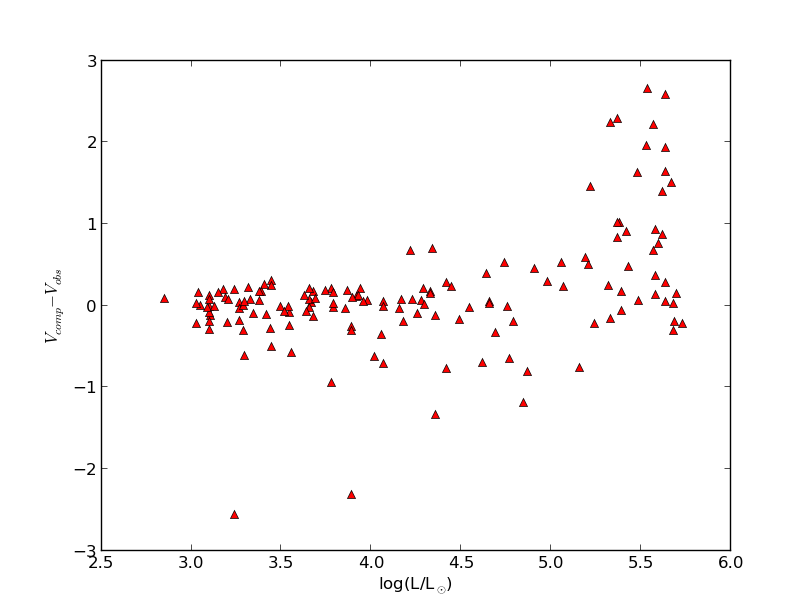
\includegraphics[width=0.9\textwidth]{diffmaglogL}
  \caption{Difference between computed and observed magnitudes as a function of $\log(L/L_\odot)$}
 \end{figure}
 
 The theoretical magnitudes ($V_{comp}$) were computed using stellar radius, luminosity and distance. The observational magnitudes ($V_{obs}$)
 were taken from a sample of 150 stars between M=5M$_\odot$ and M=48M$_\odot$ from \citep{2014A&A...570L..13C}
 
 Figure \ref{diffmagmass} shows the difference between computed and observed magnitudes as a function of mass. There is a significant
 deviation towards higher $V_{comp}$ at high masses. This can be explained using Figure \ref{castroetal}:
 \begin{figure}
  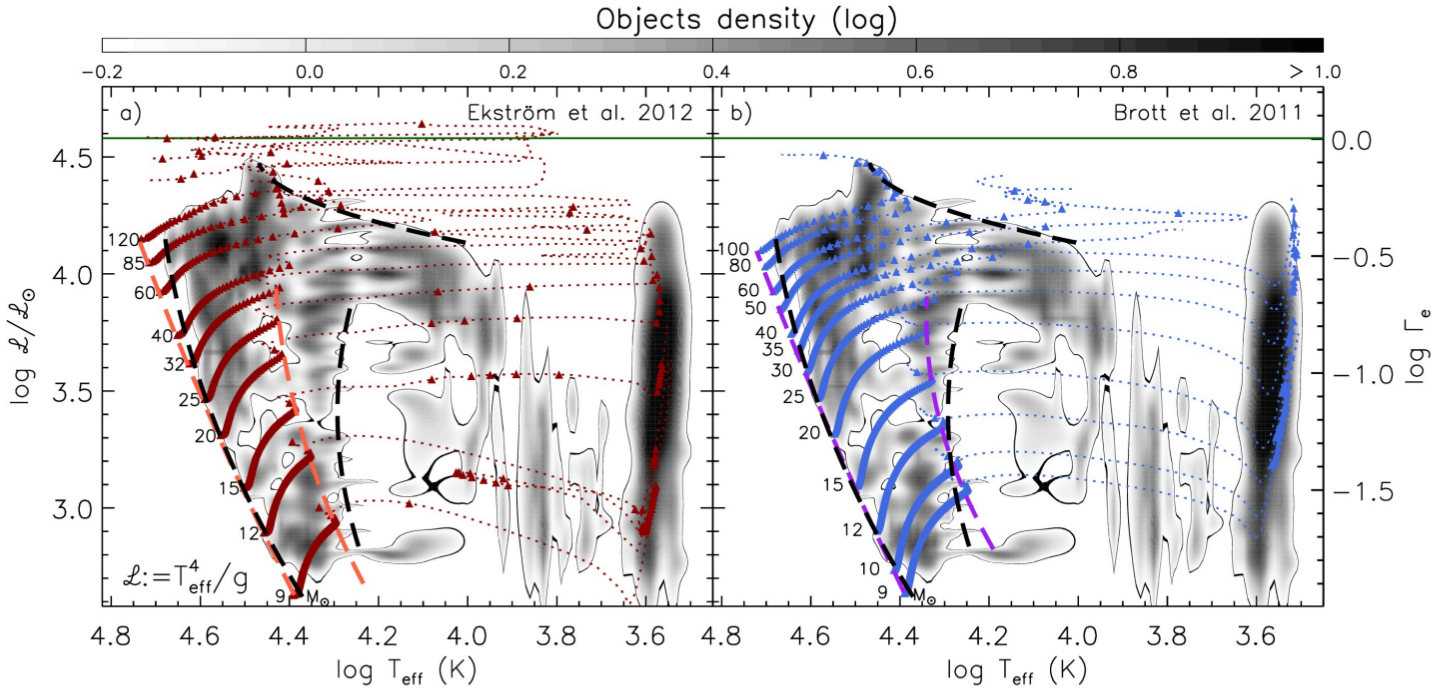
\includegraphics[width=\textwidth]{Castroetal}
  \caption{Grey scale representation of the probability density distribution of the location of 575 Galactic stars in the sHRD.
  Overlayed are stellar evolution tracks for non-rotating stars with solar composition a)\citet{2012A&A...537A.146E}
  and b)\citet{2011yCat..35309115B}. The ZAMS and TAMS positions of the models are connected through orange and purple dashed lines.
  Red and blue triangles are placed on the tracks separated by 0.1 Myr \citep{2014A&A...570L..13C}\label{castroetal}}
 \end{figure}

 My code uses an evolutionary model similar to model a). $V_{obs}$ however is obtained using a model similar to model b).
 Model b) accounts for convective overshooting to a higher degree and thus the lifetime of stars is expanded. This would account for
 minor deviations. Because of the difference in position of TAMS in the HRD, \textbf{I STILL DON'T GET IT}.
 The massive deviations between $M=25M_\odot$ and $M\approx 43M_\odot$ can be explained by taking into account inflation. 
 Near TAMS on the main sequence massive stars will undergo an expansion of their envelopes. This gives rise to a big shift on the
 HRD.
 

 
 \begin{figure}[h!]
  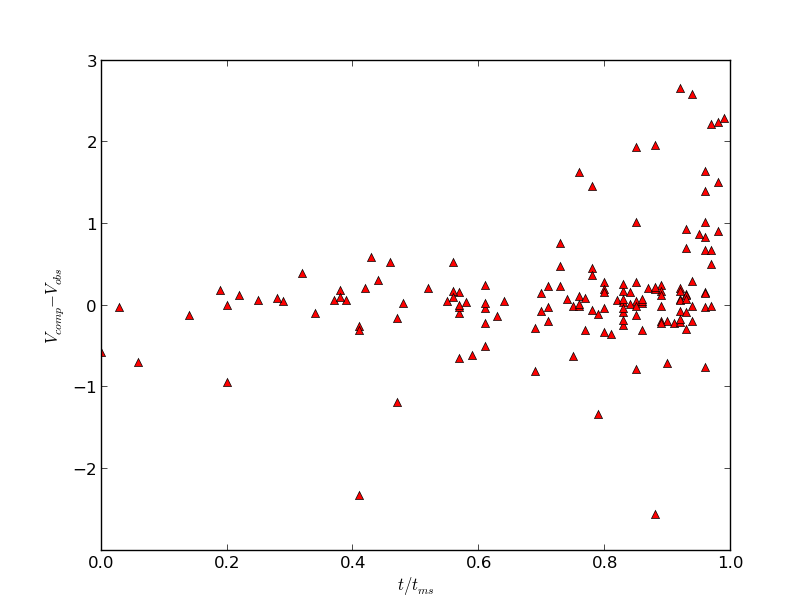
\includegraphics[width=0.9\textwidth]{diffmagfracms}
  \caption{Difference between computed and observed magnitudes as a function of age}
 \end{figure}
 
 
 
 The deviation to negative values is mostly caused by extinction. It is most prevalent in lower absolute ages. 
 Stars of lower ages are primarily found in regions of active star formation. This would mean, that they are found in regions
 of high gas density. This gas will cause extinction and thus increase $V_{obs}$. My model for extinction does not take into account 
 these density fluctuations.
 
 \newpage
 \subsection{numerical tests}
 \begin{figure}[h!]
  \begin{minipage}{0.49\textwidth}
   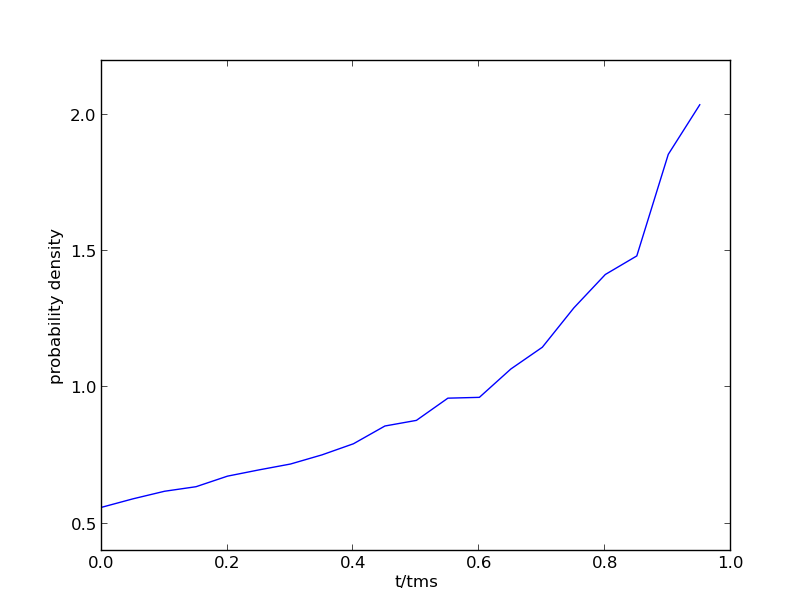
\includegraphics[width=\textwidth]{100-100-100}
  \end{minipage}
  \begin{minipage}{0.49\textwidth}
   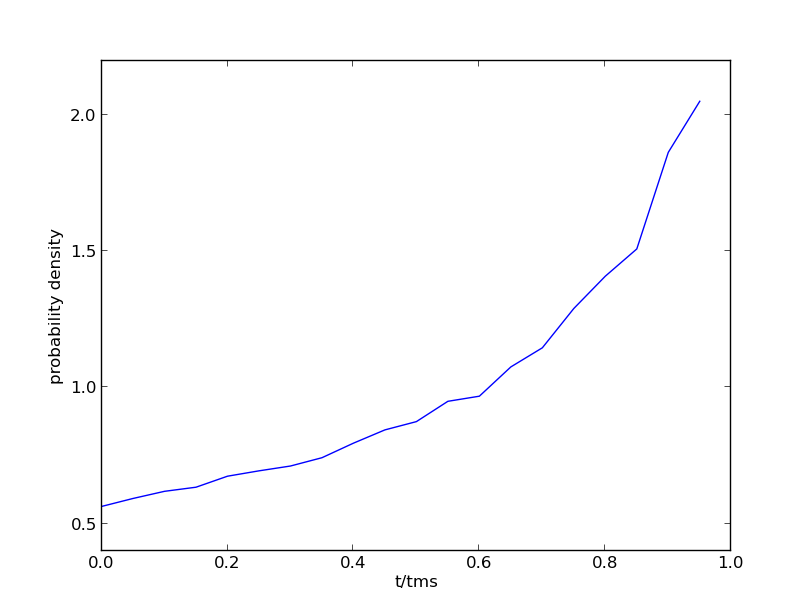
\includegraphics[width=\textwidth]{10-100-100}
  \end{minipage}
  \begin{minipage}{0.49\textwidth}
   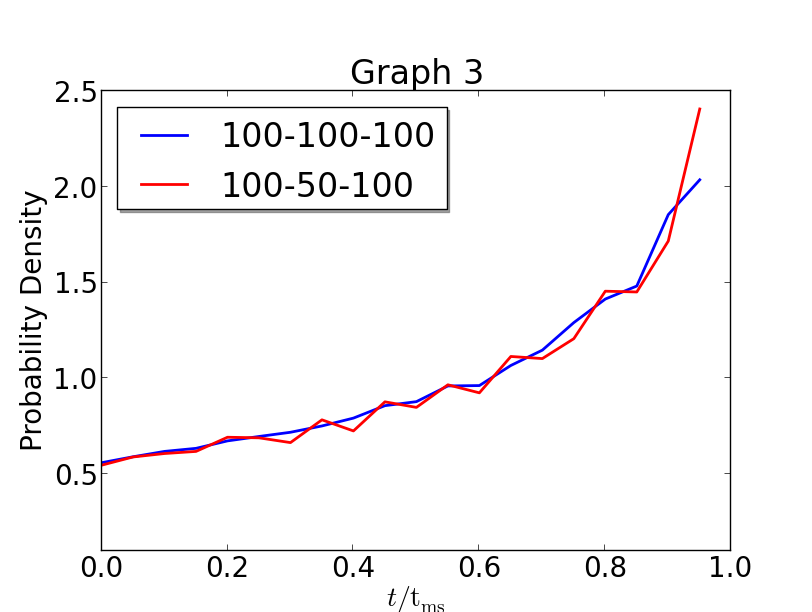
\includegraphics[width=\textwidth]{100-50-100}
  \end{minipage}
  \begin{minipage}{0.49\textwidth}
   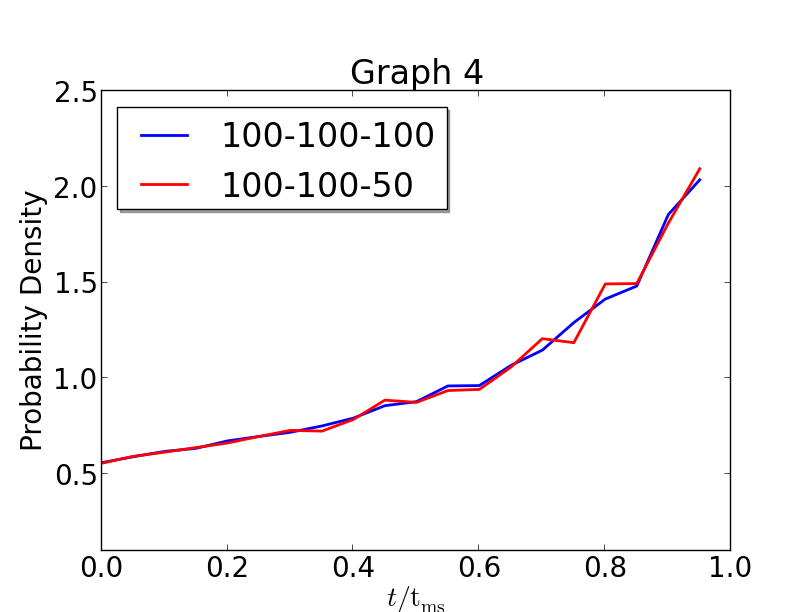
\includegraphics[width=\textwidth]{100-100-50}
  \end{minipage}
   \caption{PDF for all stars in my sample with a magnitude cut at V=9 with different binnings.
   The legend shows the binning of each line. The first value being distance, the second being mass and the third being age.\label{binnings}}
 \end{figure}
 
 Figure \ref{binnings} shows the PDF for all stars in my sample with a magnitude cut at V=9 in four graphs. 
 Graph 1 shows both the function with a resolution of 100-100-100 in distance-mass-age and the final results without noise for reference. 
 One can see from this
 graph that with this resolution there is noise that needs to be eliminated. 
 To understand what variables play the biggest part in creating this noise, in Graphs 2, 3 and 4 I change the resolution of a select 
 variable and compare the resulting curve to the curve of 100-100-100 resolution.\\
 
 In Graph 2 one can see, that even tho I cut the resolution of distance by one order of magnitude, the curves only deviate very little. This
 tells me, that distance will be very robust to a low resolution. Graphs 3 and 4, even tho I only cut the resolution in half, both 
 show a significant increase in noise, Graph 3 showing the greatest deviation from the reference-curve. Using these results, I determine 
 a binning of 100-1500-750 to yield an appropriate resolution to maximize accuracy and minimize computing time.
 
 \newpage
 \section{Results}
 \begin{figure}[h!]
   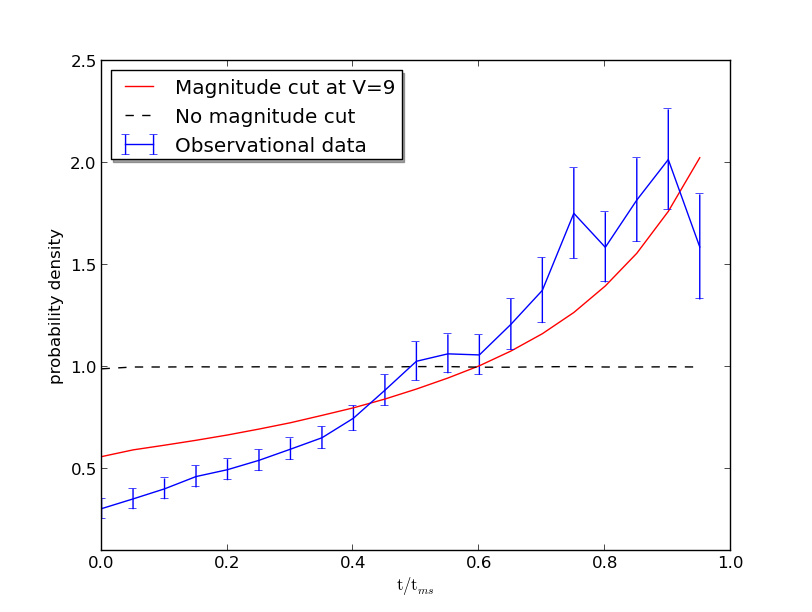
\includegraphics[width=\textwidth]{plot1}
   \caption{PDF of volume limited sample, with magnitude cut at V=9 (red line), PDF without magnitude cut
   (dashed line) and observational data with error bars (blue line). All computed data is obtained using a binning of 100-1500-750
   in distance-mass-age. The observational data is taken from Fossati et al., 2015 (in prep.).\label{all3}}
 \end{figure}
 
 Figure \ref{all3} shows the PDF with magnitude cut at V=9, PDF without magnitude cut and observational data with error bars.
 The PDF without magnitude cut shows, that the stars are uniformly distributed in $\tau$. This was expected,
 because the simluation assumes a constant star formation rate.\\
 
 Introducing a magnitude cut produces a similar trend to the one observed in the observational data. Figure \ref{magage} shows
 V as a function of fractional main sequence age for five different stars at a distance of 1$\,$kpc based on the evolutionary model of 
 \citet{2000MNRAS.315..543H}. V is a monotonic decreasing function of age.  \textbf{I need to write some more here}\\
 \begin{figure}
  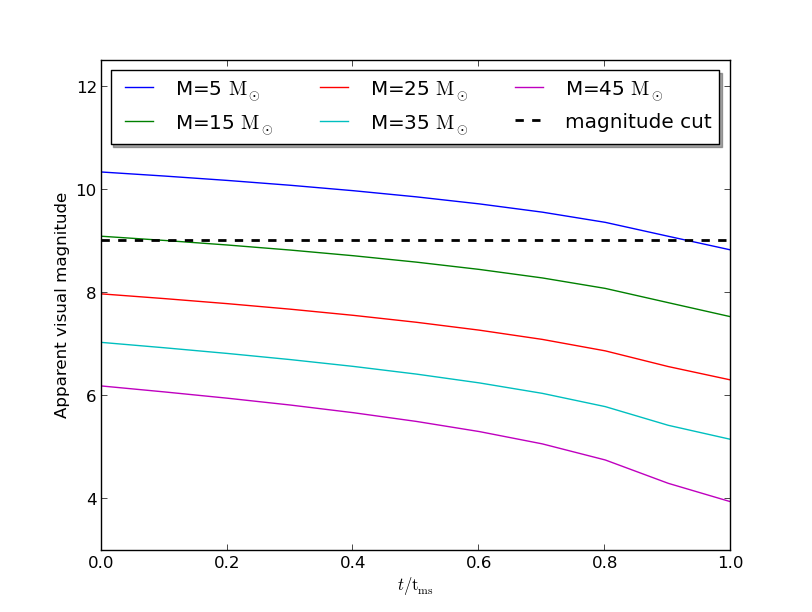
\includegraphics[width=\textwidth]{magage}
  \caption{V as a function of fractional main sequence age for five different stars at a distance of 1$\,$kpc based on the evolutionary model 
  of \citet{2000MNRAS.315..543H} The dashed line shows the magnitude cut I implemented.\label{magage}}
 \end{figure}

 There are a lot of things, that can still be implemented:\\
 \begin{itemize}
  \item Right now the stars are distributed homogenously in a sphere of a 3kpc radius. To make it more accurate one could model our
  galactic neighborhood. Namely take into account the thickness of the galactic disk, which is smaller, than 3kpc.
  \item The program does not take into account binary stars. This possibly has a major effect, because most massive stars are in binary
  systems \citep{2012Sci...337..444S}
  \item From observations we know, that we live in a part of the galaxy with little star formation.  
  The density of young open starclusters increases the farther you move away from the solar system. As seen in Figure \ref{clusters}.
  \item My model for reddening is only an approximation. It does not take into account density fluctuations in the interstellar medium. 
  The effects of which can be seen in figures \textbf{reference to diffmag}.
 \end{itemize}
 \begin{figure}[h!]
  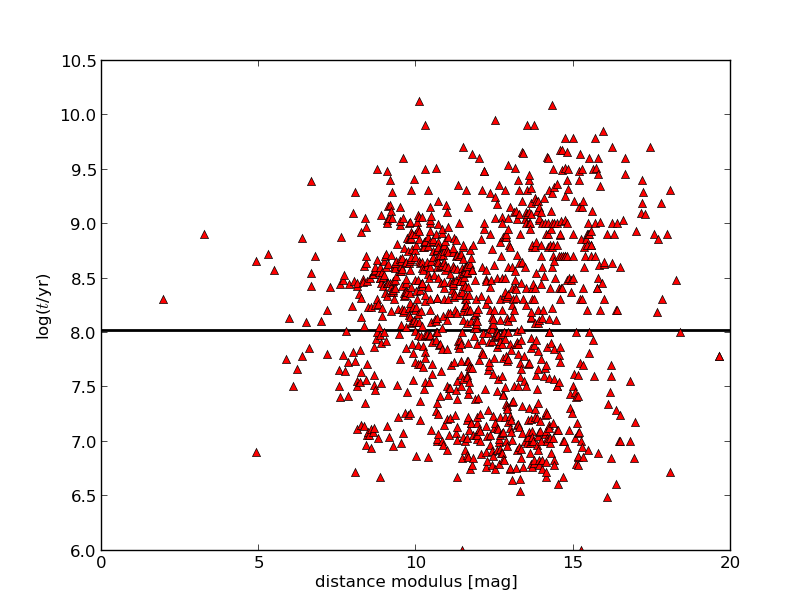
\includegraphics[width=\textwidth]{clusters}
  \caption{Open starclusters in our galaxy with distance modulus vs log(Age/yr)  \label{clusters}}
 \end{figure}

 
 \section{Conclusions}
 
 
 
 \bibliography{adssample}
\end{document}
